% Provenance (never printed): see sources/outline_sources.md (Year 3: gravity, magnetic,
% seismic, resistivity and ground-penetrating-radar surveys; data processing and
% uncertainty; a mapping project).
% Brief: sources/book5/BRIEFS.md, ch. 31. Curves from figdata/bachelor-3/gravity_granite.py
% (prism model of the Varden granite of figdata/shared/region.py), magnetic_dyke.py (2-D
% dyke; the Varden dolerite dyke of the Sync 3 ruling, buried below the unconformity),
% resistivity_sounding.py (Pekeris transform and image series) and gpr_radargram.py.
% Physical-property ranges and survey practice from the GPG open textbook (CC BY 4.0) and
% Keys (1990). Exercise and problem values in the Book 5 scratch calculator calc/ch31.py.
\chapter{Métodos de campo y de laboratorio III}\label{ch:b3:field-lab-methods-3}

Un equipo de geofísica pasa una semana en el valle de las Colinas de Varden, la
región inventada cuyo mapa geológico dibujó el volumen de primer año en su
capítulo sobre mapas geológicos. El mapa muestra un granito que aflora en
las laderas del valle, entre los esquistos, bajo la arenisca que descansa
sobre ambos. Por dónde discurre el granito bajo la cobertera, hasta dónde llega
y a qué profundidad alcanza, nadie lo ha visto. El equipo lleva un gravímetro,
dos magnetómetros, un cable de electrodos y un radar sobre un pequeño carro.
Ninguno de estos instrumentos ve una roca: cada uno mide un campo en la
superficie —la gravedad, el campo magnético, un potencial eléctrico, el eco de un pulso de radio—
que las rocas subyacentes perturban.
Al final de la semana el equipo puede dibujar el granito que nunca vio, decir
qué espesor tiene el aluvión del fondo del valle e informar de un cuerpo
magnético que ningún mapa recogía.

Este capítulo sigue esa semana. Trata cada método por turno, como una
medida con sus correcciones y como \omterm{def:b3:seismology-imaging:inverse}{problema directo} con unos pocos cuerpos
cuyos campos se pueden calcular con exactitud; a continuación expone cómo
los errores de una prospección se acumulan y por qué un solo tipo de datos
rara vez fija un modelo; y termina con la prospección de Varden, donde
se combinan los métodos.

\begin{recall}
La anomalía de la gravedad, las correcciones y anomalías de aire libre y de Bouguer
y la gravedad normal están en el volumen de primer año, en su capítulo sobre isostasia
y gravedad; el circuito de medida de un \omterm{def:b3:field-lab-methods-3:gravimeter}{gravímetro relativo} se describe en
el \cref{ch:b3:gravity-geodesy}. El campo principal, su inclinación, la
\omterm{thm:b3:palaeomagnetism:dipole}{fórmula del dipolo} y el \omterm{def:b3:palaeomagnetism:igrf}{Campo Geomagnético Internacional de Referencia} están en
el \cref{ch:b3:palaeomagnetism}. La resistividad, la ley de Ohm, la
permitividad relativa, las ondas electromagnéticas, la imantación y la
susceptibilidad magnética están en los libros de física, y el teorema de Gauss
para la gravedad, junto con ellos. Las prospecciones sísmicas de refracción están en
el \cref{ch:b3:exploration-seismology}; los \omterm{def:b3:seismology-imaging:inverse}{problemas directo} e inverso y los
mínimos cuadrados ponderados en el \cref{ch:b3:seismology-imaging}; la porosidad en
los libros escolares y los \omterm{def:b3:facies-models:wireline}{registros de pozo} en el \cref{ch:b3:facies-models}. La
propagación de incertidumbres se trata en los libros de química y de matemáticas.
\end{recall}

\section{Prospecciones gravimétricas}\label{sec:b3:field-lab-methods-3:gravity}

Las anomalías que busca una prospección gravimétrica son pequeñas. La gravedad en el
ecuador es de unos \qty{978000}{\milli\gal}; las estructuras grandes la modifican
en cientos de miligales, un domo de sal en unos diez, un cuerpo de mena en
alrededor de uno, y los objetivos de una prospección geotécnica en unas pocas
centésimas. Los geofísicos miden en
miligales, o en unidades de \qty{0.1}{\milli\gal}; una prospección útil
debe resolver diferencias de una parte en cien millones de~$g$.
% ledger: gpg:grav-units, gpg:grav-sizes

\begin{definition}[Gravímetro relativo; deriva instrumental]\label{def:b3:field-lab-methods-3:gravimeter}
Un \emph{gravímetro relativo}\index{gravímetro relativo} es un
instrumento que mide diferencias de gravedad entre estaciones: una
masa sujeta a un muelle, mantenida en posición nula mediante una segunda fuerza
ajustable, cuya lectura en el dial, multiplicada por una constante de calibración, da
la gravedad en miligales salvo una constante desconocida. Su \emph{deriva
instrumental}\index{deriva instrumental} es el cambio lento de su lectura en una
estación fija, causado por la fluencia del muelle, la temperatura y los
golpes; se mide volviendo a leer, al cabo de unas horas, una estación ya leída, la
\emph{estación base}.
\end{definition}
% ledger: gpg:gravimeter, gpg:grav-survey

Un gravímetro de campo cubre un rango de varias decenas de miles de
miligales y lee, en su mejor caso, hasta unos \qty{0.01}{\milli\gal}; el
rango debe reajustarse tras el transporte. Con esa precisión, la altura de
cada estación importa tanto como su lectura: un error de altura de \qty{3.3}{cm}
estropea \qty{0.01}{\milli\gal}, así que las posiciones se determinan con
receptores de satélite o un nivel hasta el centímetro. La estación base se
vuelve a ocupar cada dos horas. La marea terrestre, que puede alcanzar
\qty{0.3}{\milli\gal}, cambia con suficiente lentitud en esas horas como para
eliminarse con la deriva.
% ledger: gpg:gravimeter, gpg:grav-survey, gpg:grav-sizes

\begin{method}[Reducción de un circuito gravimétrico]\label{met:b3:field-lab-methods-3:loop}
Un circuito empieza y termina en una estación base, leída en los instantes $t_0$ y $t_1$.
\begin{enumerate}
  \item Se calcula la tasa de deriva $(r_1 - r_0)/(t_1 - t_0)$ a partir de las dos
        lecturas de la base; incluye la marea.
  \item Se resta de cada lectura la deriva acumulada desde $t_0$,
        $r - (t - t_0)(r_1 - r_0)/(t_1 - t_0)$, y se resta la lectura
        de la base: así se obtiene la gravedad relativa a la estación base.
  \item Se corrige por la altura $\Delta h$ de la estación sobre la base:
        se suma la corrección de aire libre $\qty{0.3086}{\milli\gal.m^{-1}}
        \times\Delta h$ y se resta la corrección de Bouguer
        $\qty{0.1119}{\milli\gal.m^{-1}}\times\Delta h$ (densidad
        \qty{2670}{kg.m^{-3}}), es decir, se suma $0.1967\,\Delta h$.
  \item Para una estación situada a una distancia $\Delta y$ al norte de la base, se resta
        la variación de la gravedad normal, $\qty{0.811}{\milli\gal.km^{-1}}
        \times\sin 2\varphi\times\Delta y$.
  \item Se suma la \omterm{def:b3:field-lab-methods-3:terrain}{corrección topográfica} de cada estación.
\end{enumerate}
El resultado es la anomalía de Bouguer relativa a la base. Si se liga la base
a una estación de gravedad absoluta conocida se obtiene la anomalía misma.
\end{method}
% ledger: gpg:grav-survey, gpg:terrain

La corrección de Bouguer trata el terreno comprendido entre la estación y el
nivel de referencia como una losa plana. En un relieve real esto es erróneo de dos maneras:
una colina que se eleva sobre la estación atrae hacia arriba y reduce la
lectura, y un valle que queda por debajo se cuenta en la losa como
roca que no está allí.

\begin{definition}[Corrección topográfica]\label{def:b3:field-lab-methods-3:terrain}
La \emph{corrección topográfica}\index{corrección topográfica} de una estación de gravedad
es la atracción que ejercen sobre ella las desviaciones del relieve respecto de la
losa de Bouguer: las colinas por encima del nivel de la estación y
los valles por debajo de él, contados con la densidad de la losa. Ambos
reducen la gravedad medida frente a la losa, por lo que la corrección se
suma siempre.
\end{definition}

Antiguamente se calculaba a mano, con un ábaco de Hammer y tablas, zona por zona
hacia fuera desde la estación; hoy se calcula a partir de un modelo digital
de elevaciones. Lejos de los relieves escarpados rara vez supera \qty{1}{\milli\gal},
pero las zonas próximas a la estación son difíciles de acertar, y la
corrección rara vez se conoce con una precisión mejor que \qty{0.2}{\milli\gal}.
% ledger: gpg:terrain, gpg:grav-sizes

\subsection{Anomalías de cuerpos simples}

El \omterm{def:b3:seismology-imaging:inverse}{problema directo} de la gravedad es una suma: cada elemento de un cuerpo de
contraste de densidad $\Delta\rho$ atrae a la estación según la ley de Newton, y
una prospección mide la componente vertical de la suma. Unos pocos cuerpos la dan
en forma cerrada.

\begin{theorem}[Esfera y cilindro horizontal]\label{thm:b3:field-lab-methods-3:sphere}
A una distancia horizontal $x$ del punto situado sobre su centro, una esfera enterrada
de exceso de masa $\Delta m$ cuyo centro está a profundidad $z$ produce la
anomalía
\[
\Delta g(x) = \frac{G\,\Delta m\,z}{(x^2 + z^2)^{3/2}} ,
\]
y la anomalía cae a la mitad de su máximo en $x_{1/2} = z\sqrt{2^{2/3} - 1}$,
de modo que $z = 1.305\,x_{1/2}$. Un cilindro horizontal largo de exceso de masa
$\lambda$ por unidad de longitud, con su eje a profundidad $z$, produce, transversalmente a su
rumbo
\[
\Delta g(x) = \frac{2G\lambda z}{x^2 + z^2} ,
\]
y $z = x_{1/2}$.
\end{theorem}

\begin{proof}
Fuera de una esfera cuya densidad depende solo de la distancia a su
centro, la atracción es la de su masa concentrada en el centro (el
teorema de las capas esféricas, consecuencia del teorema de Gauss). Su módulo en la
estación es $G\Delta m/(x^2 + z^2)$, y la componente vertical lleva el
factor $z/\sqrt{x^2 + z^2}$. Escribiendo $\Delta g(x_{1/2}) =
\Delta g(0)/2$ se obtiene $(1 + x_{1/2}^2/z^2)^{3/2} = 2$, de donde sale la regla. Para
el cilindro, el teorema de Gauss aplicado a un cilindro coaxial de radio $r$ da
un campo $2G\lambda/r$, y la componente vertical $2G\lambda z/r^2$;
la mitad del máximo se alcanza cuando $x^2 + z^2 = 2z^2$.
\end{proof}
% ledger: gpg:half-width

Un cuerpo que no es esférico también tiene una semianchura, y la regla
proporciona entonces la profundidad de una esfera equivalente, no la del cuerpo. La regla es
una primera estimación, hecha antes de ajustar ningún modelo.

\begin{proposition}[Cilindro vertical sobre su eje]\label{prop:b3:field-lab-methods-3:vcyl}
Un cilindro vertical de radio $a$ y contraste de densidad $\Delta\rho$,
cuyo techo y cuya base están a profundidades $z_1 < z_2$ bajo la estación,
produce sobre su eje
\[
\Delta g = 2\pi G\Delta\rho\left[(z_2 - z_1) + \sqrt{z_1^2 + a^2}
           - \sqrt{z_2^2 + a^2}\right] .
\]
Para $a \to \infty$ es la losa de Bouguer $2\pi G\Delta\rho(z_2 - z_1)$;
para un cilindro desde la superficie hasta gran profundidad tiende a
$2\pi G\Delta\rho\,a$.
\end{proposition}

\begin{proof}
Un disco de radio $a$ y espesor $\mathrm{d}z$ a profundidad $z$ atrae
a un punto de su eje mediante $2\pi G\Delta\rho\,\mathrm{d}z\,(1 -
z/\sqrt{z^2 + a^2})$, la atracción de un anillo integrada sobre el
radio. Integrando de $z_1$ a $z_2$ se obtiene el corchete. Cuando $a \to
\infty$ con profundidades fijas, $\sqrt{z_1^2 + a^2} - \sqrt{z_2^2 + a^2} =
(z_1^2 - z_2^2)/(\sqrt{z_1^2 + a^2} + \sqrt{z_2^2 + a^2}) \to 0$; cuando
$z_1 = 0$ y $z_2 \to \infty$, $z_2 - \sqrt{z_2^2 + a^2} \to 0$ y
el corchete tiende a $a$.
\end{proof}

\begin{proposition}[Exceso de masa a partir de un mapa gravimétrico]\label{prop:b3:field-lab-methods-3:gauss}
Sea cual sea la forma de un cuerpo que yace por completo bajo un
plano horizontal, su exceso de masa es
\[
\Delta m = \frac{1}{2\pi G}\iint \Delta g\,\mathrm{d}A ,
\]
siendo la integral extendida a todo el plano.
\end{proposition}

\begin{proof}
\sloppy Para una masa puntual $m$ a profundidad $z$, siendo $r$ la distancia horizontal,
$\iint \Delta g\,\mathrm{d}A = \int_0^\infty
Gmz\,(r^2 + z^2)^{-3/2}\,2\pi r\,\mathrm{d}r = 2\pi Gm$: la mitad del flujo
$4\pi Gm$ del teorema de Gauss atraviesa el plano. Un cuerpo es una suma de masas
puntuales, y la integral es lineal.
\end{proof}

El teorema proporciona la masa, nunca la forma; y un mapa cubre solo parte
del plano, mientras que la anomalía de un cuerpo profundo decae lentamente, de modo que
la masa obtenida a partir de un mapa resulta demasiado pequeña a menos que sus bordes se prolonguen
mediante un modelo.

\begin{omfigure}
\begin{tikzpicture}
\begin{axis}[axis equal image, xmin=1.5, xmax=5.5, ymin=2.6, ymax=5.7, width=0.86\linewidth,
  tick label style={font=\scriptsize}, xlabel={este (km)}, ylabel={norte (km)},
  label style={font=\small}, unbounded coords=jump]
% geology of the region (figdata/shared/region.py), faded
\addplot[lith schist, draw=black!50, line width=0.2pt, even odd rule, opacity=0.45] table {figdata/out/shared-region-unit-schist.dat};
\addplot[lith granite, draw=black!50, line width=0.2pt, even odd rule, opacity=0.45] table {figdata/out/shared-region-unit-granite.dat};
\addplot[om lith={icsTriassic!35}{om sand}, draw=black!50, line width=0.2pt, even odd rule, opacity=0.45] table {figdata/out/shared-region-unit-sandstone.dat};
\addplot[om lith={icsJurassic!40}{om limestone}, draw=black!50, line width=0.2pt, even odd rule, opacity=0.45] table {figdata/out/shared-region-unit-limestone.dat};
\addplot[om lith={icsJurassic!15}{om shale}, draw=black!50, line width=0.2pt, even odd rule, opacity=0.45] table {figdata/out/shared-region-unit-shale.dat};
\addplot[lith alluvium, draw=black!50, line width=0.2pt, even odd rule, opacity=0.45] table {figdata/out/shared-region-unit-alluvium.dat};
\addplot[river] table {figdata/out/shared-region-river.dat};
% the survey (figdata/bachelor-3/gravity_granite.py, magnetic_dyke.py)
\addplot[only marks, mark=*, mark size=0.7pt, black!70] table[x=x_km, y=y_km] {figdata/out/bachelor-3-gravity_granite-stations.dat};
\addplot[omDef, very thick] table[x=x_km, y=y_km] {figdata/out/bachelor-3-gravity_granite-contours.dat};
\addplot[omThm, thick] coordinates {(1.5,4.15) (5.5,4.15)};
\addplot[omMeth, line width=2.2pt, opacity=0.8] coordinates {(1.7,4.15) (2.7,4.15)};
\addplot[omProp, dashed, thick] coordinates {(2.2,2.6) (2.2,5.7)};
\addplot[only marks, mark=star, mark size=3.5pt, omMeth!70!black, thick] coordinates {(3.5,4.0)};
\node[font=\scriptsize, fill=white, fill opacity=0.85, text opacity=1, inner sep=1pt] at (axis cs:3.5,5.12) {$-0.5$};
\node[font=\scriptsize, fill=white, fill opacity=0.85, text opacity=1, inner sep=1pt] at (axis cs:3.5,4.84) {$-1$};
\node[font=\scriptsize, fill=white, fill opacity=0.85, text opacity=1, inner sep=1pt] at (axis cs:3.5,4.58) {$-2$};
\node[font=\scriptsize, anchor=south west, fill=white, fill opacity=0.85, text opacity=1, inner sep=1pt] at (axis cs:1.55,4.17) {perfil gravimétrico};
\node[font=\scriptsize, anchor=north, fill=white, fill opacity=0.85, text opacity=1, inner sep=1pt] at (axis cs:2.2,4.08) {línea magnética};
\node[font=\scriptsize, anchor=north west, text=omProp!80!black, fill=white, fill opacity=0.85, text opacity=1, inner sep=1pt] at (axis cs:2.24,5.6) {dique enterrado};
\node[font=\scriptsize, anchor=north, fill=white, fill opacity=0.85, text opacity=1, inner sep=1pt] at (axis cs:3.5,3.92) {sondeo};
\pic at (axis cs:5.15,5.3) {northarrow};
\end{axis}
\end{tikzpicture}

\par\smallskip{\small La prospección de Varden sobre el mapa geológico de la región
(atenuado: esquisto gris, granito rosa, arenisca, caliza y lutita de la
cobertera, depósitos aluviales a lo largo del río). Puntos negros: las estaciones gravimétricas,
\qty{200}{m} de separación; azul: la anomalía de Bouguer del modelo de granito,
con isolíneas cada \qty{0.5}{\milli\gal}; rojo: el perfil gravimétrico; verde:
la línea magnética y el sondeo eléctrico (estrella) en el
fondo del valle; naranja a trazos: el dique de dolerita que la prospección magnética detecta,
enterrado bajo la cobertera.}\label{fig:b3:field-lab-methods-3:survey}
\end{omfigure}
% ledger: gpg:densities

\subsection{El granito de Varden}

El modelo que los geólogos proponen para el granito es un cuerpo elíptico situado bajo la
discordancia, con \qty{760}{m} de extensión este--oeste y \qty{1120}{m}
en dirección norte--sur donde contacta con la cobertera, ensanchándose hacia abajo; en las
laderas del valle alcanza la superficie. El granito es más ligero que el esquisto:
los intervalos de densidad publicados son \numrange{2.50}{2.81} y
\qtyrange{2.39}{2.80}{g.cm^{-3}}. El modelo de la prospección adopta
\qty{2620}{kg.m^{-3}} para el granito y \qty{2750}{kg.m^{-3}} para el
esquisto, un contraste de \qty{-130}{kg.m^{-3}}, y detiene el granito a
\qty{1500}{m} bajo el nivel del mar, una suposición, ya que nada muestra su
base. Se divide en \num{5533} prismas rectos cuyas atracciones tienen una
forma cerrada, el modelo da la anomalía del mapa anterior: un mínimo cerrado de
\qty{-2.29}{\milli\gal} sobre el centro del granito, con sus isolíneas
alargadas en sentido norte--sur, como el cuerpo.
% ledger: gpg:densities

\begin{omfigure}
\begin{tikzpicture}
\begin{axis}[width=0.8\linewidth, height=0.42\linewidth, xmin=1.5, xmax=5.5, ymin=-2.6, ymax=0.2,
  xlabel={este (km)}, ylabel={$\Delta g$ (\unit{\milli\gal})},
  tick label style={font=\scriptsize}, label style={font=\small},
  legend style={font=\scriptsize, at={(0.02,0.04)}, anchor=south west}]
% computed in figdata/bachelor-3/gravity_granite.py
\addplot[omDef, very thick] table[x=x_km, y=dg_mGal] {figdata/out/bachelor-3-gravity_granite-profile.dat};
\addlegendentry{modelo de granito}
\addplot[omThm, densely dashed, thick] table[x=x_km, y=sphere] {figdata/out/bachelor-3-gravity_granite-profile.dat};
\addlegendentry{esfera de la regla de la semianchura}
\addplot[omMeth, densely dotted, thick] table[x=x_km, y=cyl] {figdata/out/bachelor-3-gravity_granite-profile.dat};
\addlegendentry{cilindro vertical}
\addplot[black!40, forget plot] coordinates {(1.5,0) (5.5,0)};
\addplot[black!50, densely dotted, forget plot] coordinates {(1.5,-1.1464) (5.5,-1.1464)};
\node[font=\scriptsize, black!60, anchor=south east] at (axis cs:5.45,-1.14) {la mitad del pico};
\end{axis}
\end{tikzpicture}

\par\smallskip{\small La anomalía a lo largo del perfil gravimétrico (azul), la
esfera cuya profundidad y masa obtiene la regla de la semianchura (roja a trazos), y
un cilindro vertical de la misma área que el granito en la discordancia,
desde el terreno hasta la base del modelo (en verde, punteado). La esfera coincide
con el pico y la semianchura por construcción, pero no con los flancos; el
cilindro, que ignora el ensanchamiento del cuerpo, no alcanza el valor en el
centro.}\label{fig:b3:field-lab-methods-3:profile}
\end{omfigure}
% ledger: gpg:half-width

\section{Prospecciones magnéticas}\label{sec:b3:field-lab-methods-3:magnetics}

El campo principal de la Tierra es de unos \qty{25000}{nT} en el ecuador magnético
y de unos \qty{70000}{nT} cerca de los polos magnéticos. Las rocas que contienen
magnetita añaden su propio campo a este, inducido por el campo principal en
proporción a su susceptibilidad, o remanente, adquirido desde el momento
en que se formaron. Una roca ígnea félsica tiene una susceptibilidad inferior a unos
\num{2e-3}, mientras que una máfica tiene entre unos \num{2e-3} y \num{0.4}; en la misma
escala, el 1 por ciento de magnetita en volumen da unos \num{0.03}.
% ledger: gpg:mag-field, gpg:susceptibility

\begin{definition}[Anomalía de campo total; corrección diurna; reducción al polo]\label{def:b3:field-lab-methods-3:magnetic}
Sea $\mathbf{F}$ el campo principal en la prospección y $\Delta\mathbf{B}$
el campo de las rocas magnetizadas.
\begin{itemize}
  \item La \emph{anomalía de campo total}\index{anomalía de campo total} es
        la intensidad medida menos la del campo principal, $\Delta T =
        |\mathbf{F} + \Delta\mathbf{B}| - |\mathbf{F}|$; cuando
        $|\Delta\mathbf{B}| \ll |\mathbf{F}|$ es la proyección
        $\Delta\mathbf{B}\cdot\mathbf{F}/|\mathbf{F}|$.
  \item La \emph{corrección diurna}\index{corrección diurna} elimina
        las variaciones del campo con el tiempo: un magnetómetro en una estación base
        fija registra el campo durante toda la prospección, y cada
        lectura $T(t)$ del instrumento móvil se sustituye por $T(t) -
        T_\mathrm{base}(t)$.
  \item La \emph{reducción al polo}\index{reducción al polo}
        calcula, a partir de la anomalía medida, la que darían las mismas rocas
        si el campo principal fuera vertical, como en un polo
        magnético; la anomalía queda entonces situada sobre su fuente.
\end{itemize}
\end{definition}
% ledger: gpg:mag-survey, gpg:mag-processing

Las variaciones con el tiempo proceden de corrientes en la ionosfera, a unos
\qty{110}{km} de altura. En un día suelen alcanzar unos
\qtyrange{20}{50}{nT}, tanto como la anomalía de un objetivo pequeño; una
tormenta magnética puede cambiar el campo en miles de nanoteslas. La
estación base mide la variación, suponiendo que es la
misma en toda la prospección. El propio campo principal, o el campo de
estructuras más grandes que la prospección, se elimina con el IGRF, una constante
o una tendencia ajustada.
% ledger: gpg:mag-field, gpg:mag-processing

Un magnetómetro de precesión protónica mide la frecuencia a la que precesan
los espines de los protones en el campo, que es proporcional a este; el aparato
lee con una resolución de \qty{1}{nT} y necesita más de un segundo por lectura. Un
magnetómetro de cesio de bombeo óptico es entre diez y cien veces más
sensible, y lee hasta \qty{0.01}{nT}. Las estaciones deben estar lo bastante
juntas para colocar al menos unas tres lecturas a lo largo de la semianchura de la
anomalía más estrecha que se busca, y cuanto más somera sea la fuente, más próximas
deben estar.
% ledger: gpg:mag-survey

\begin{proposition}[Anomalía de un dique delgado]\label{prop:b3:field-lab-methods-3:dyke}
Un dique vertical de espesor $t$ y susceptibilidad $\kappa$, con rumbo
a lo largo del meridiano magnético, con su techo a profundidad $z$ y extendiéndose
muy hacia abajo, imantado por inducción en un campo principal $F$ de inclinación $I$,
produce, transversalmente a su rumbo, si $t \ll z$,
\[
\Delta T(x) = \frac{\kappa F t\sin^2 I}{2\pi}\,\frac{z}{x^2 + z^2} ,
\]
una anomalía simétrica que cae a la mitad de su pico en $x = \pm z$: la
profundidad del techo del dique es la mitad de la anchura total de la anomalía a
la mitad de su pico.
\end{proposition}

\begin{proof}
El dique es bidimensional y el campo principal yace en el plano vertical
del rumbo. La imanación $\mathbf{M} = \kappa\mathbf{F}/\mu_0$
tiene una componente a lo largo del rumbo, cuyos polos quedan en los extremos del
dique, lejanos, y que no produce campo; y una componente vertical $M
\sin I$, que sitúa en la cara superior del dique una carga magnética de
$-Mt\sin I$ por unidad de longitud (con $\mathbf{M}\cdot\mathbf{n}$ como la
densidad de carga, $\mathbf{n}$ la normal saliente), estando la cara inferior
alejada. Una carga lineal $q$ por unidad de longitud produce, por el teorema de Gauss
en dos dimensiones, un campo $q/(2\pi r)$ a lo largo del radio. En una
estación en $(x, 0)$ situada sobre un techo en $(0, z)$, su componente hacia abajo es
$Mt\sin I\,z/(2\pi(x^2 + z^2))$, y su componente horizontal es
transversal al rumbo, perpendicular a $\mathbf{F}$. Multiplicando por
$\mu_0$ y proyectando sobre $\mathbf{F}$, cuya componente vertical es
$\sin I$, se obtiene $\Delta T$. La condición de mitad de pico es $x^2 + z^2 =
2z^2$.
\end{proof}

Cuando el dique tiene rumbo transversal al meridiano, las partes horizontales de la
imanación y del campo principal yacen ambas en el plano del
perfil, las caras laterales portan cargas, y la anomalía se vuelve
asimétrica, con un mínimo del lado del polo. La figura siguiente
la calcula de forma exacta para un dique de anchura finita, sumando los campos cerrados
de sus cuatro caras cargadas. La \omterm{def:b3:field-lab-methods-3:magnetic}{reducción al polo} convierte tal
anomalía de nuevo en la simétrica de un campo vertical.

\begin{omfigure}
\begin{tikzpicture}
\begin{groupplot}[group style={group size=2 by 1, horizontal sep=1.5cm},
  width=0.48\linewidth, height=0.42\linewidth,
  tick label style={font=\scriptsize}, label style={font=\small}, title style={font=\small}]
\nextgroupplot[xmin=-600, xmax=600, ymin=-6, ymax=28, xlabel={distancia (\unit{m})},
  ylabel={$\Delta T$ (\unit{nT})}, title={un dique a dos inclinaciones},
  scaled x ticks=false,
  legend style={font=\scriptsize, at={(0.98,0.98)}, anchor=north east}]
% computed in figdata/bachelor-3/magnetic_dyke.py
\addplot[omDef, very thick] table[x=x_m, y=dT_I90] {figdata/out/bachelor-3-magnetic_dyke-generic.dat};
\addlegendentry{$I = 90^\circ$}
\addplot[omThm, thick] table[x=x_m, y=dT_I60] {figdata/out/bachelor-3-magnetic_dyke-generic.dat};
\addlegendentry{$60^\circ$, rumbo E--O}
\addplot[omMeth, densely dashed, thick] table[x=x_m, y=dT_I60ns] {figdata/out/bachelor-3-magnetic_dyke-generic.dat};
\addlegendentry{$60^\circ$, rumbo N--S}
\addplot[black!40, forget plot] coordinates {(-600,0) (600,0)};
\node[font=\scriptsize, black!60, anchor=south west] at (axis cs:-590,-5.6) {sur};
\node[font=\scriptsize, black!60, anchor=south east] at (axis cs:590,-5.6) {norte};
\nextgroupplot[xmin=1.7, xmax=2.7, ymin=0, ymax=40, xlabel={este (km)},
  ylabel={campo $- \qty{48000}{nT}$}, title={la línea de Varden, tal como se lee},
  legend style={font=\scriptsize, at={(0.02,0.98)}, anchor=north west}]
\addplot[omDef, thick, mark=*, mark size=1.1pt] table[x=x_km, y expr=\thisrow{T_obs}-48000] {figdata/out/bachelor-3-magnetic_dyke-line.dat};
\addlegendentry{instrumento en movimiento}
\addplot[omThm, thick, densely dashed] table[x expr=1.7+\thisrow{t_min}/40, y expr=\thisrow{T_base}-48000] {figdata/out/bachelor-3-magnetic_dyke-base.dat};
\addlegendentry{estación base}
\end{groupplot}
\end{tikzpicture}

\par\smallskip{\small Izquierda: la \omterm{def:b3:field-lab-methods-3:magnetic}{anomalía de campo total} de un dique vertical
\qty{20}{m} de espesor, con su techo a \qty{100}{m} de profundidad, susceptibilidad \num{0.01},
en un campo de \qty{50000}{nT}; en perfiles transversales a un rumbo este--oeste,
con inclinaciones de \ang{90} y \ang{60}, y transversales a un rumbo norte--sur
a \ang{60}. Derecha: las lecturas a lo largo de la línea magnética de Varden,
una estación cada \qty{50}{m} y una cada dos minutos, de oeste a este,
y la estación base en los mismos instantes (representada en la posición que
ocupaba entonces el instrumento móvil): el ascenso diurno del campo equivale a la
mitad del tamaño de la anomalía.}\label{fig:b3:field-lab-methods-3:magnetic}
\end{omfigure}
% ledger: gpg:mag-field, gpg:susceptibility

\section{Métodos eléctricos}\label{sec:b3:field-lab-methods-3:electrical}

La resistividad abarca un intervalo más amplio que cualquier otra propiedad de las rocas:
las rocas ígneas y metamórficas no alteradas se sitúan entre unos
\num{1000} y \qty{100000}{\ohm\metre}, las lutitas entre unos
\num{3} y \num{30}, la grava y la arena secas entre unos pocos cientos y diez
mil; el agua dulce se sitúa entre unos \num{1.5} y
\qty{130}{\ohm\metre}, y el agua salada por debajo de uno. El agua de los poros conduce
mejor que la mayoría de los minerales formadores de rocas, gracias a sus iones, de modo que la corriente
circula principalmente por los poros, y la porosidad, la saturación y
la salinidad del agua controlan la resistividad de una roca.
% ledger: gpg:resistivity, gpg:conduction

\begin{theorem}[Fuente puntual en un terreno uniforme]\label{thm:b3:field-lab-methods-3:point-source}
Una corriente $I$ inyectada en un punto de la superficie de un terreno uniforme de
resistividad $\rho$ produce a una distancia $r$ el potencial
\[
V(r) = \frac{\rho I}{2\pi r} .
\]
Con dos electrodos de corriente A~($+I$) y B~($-I$) y dos electrodos de potencial
M y N, la diferencia de potencial medida es
\[
\Delta V_{MN} = \frac{\rho I}{2\pi}\left(\frac{1}{AM} - \frac{1}{BM}
               - \frac{1}{AN} + \frac{1}{BN}\right) .
\]
\end{theorem}

\begin{proof}
Por simetría, la corriente fluye radialmente y atraviesa cada hemisferio de
radio $r$, de área $2\pi r^2$, de manera uniforme: $j = I/(2\pi r^2)$. La ley de Ohm
da el campo $E = \rho j$, y $V(r) = \int_r^\infty E\,\mathrm{d}r'
= \rho I/(2\pi r)$, tomando $V = 0$ a gran distancia. Los potenciales de los dos
electrodos se suman.
\end{proof}

\begin{definition}[Resistividad aparente; configuración de electrodos; sondeo eléctrico vertical; tomografía de resistividad eléctrica]\label{def:b3:field-lab-methods-3:resistivity}
\leavevmode
\begin{itemize}
  \item La \emph{resistividad aparente}\index{resistividad aparente} de una
        medida de cuatro electrodos es $\rho_a = K\,\Delta V_{MN}/I$, con
        el factor geométrico $K = 2\pi/(1/AM - 1/BM - 1/AN + 1/BN)$: la
        resistividad del terreno homogéneo que daría la misma
        lectura.
  \item Una \emph{configuración de electrodos}\index{configuración de electrodos} es una regla que
        dispone los cuatro electrodos: la configuración \emph{Wenner} los sitúa
        equiespaciados, a distancia $a$ entre sí, en el orden AMNB; la
        configuración \emph{Schlumberger} sitúa M y N, separados $2l$, en el centro
        de un AB mucho más largo, de semilongitud $s$; las configuraciones dipolo--dipolo,
        polo--dipolo y polo--polo separan el par de corriente
        del par de potencial, o envían un electrodo muy lejos.
  \item Un \emph{sondeo eléctrico vertical}\index{sondeo eléctrico vertical}
        amplía una configuración alrededor de un centro fijo y representa
        $\rho_a$ frente a la separación en escalas logarítmicas: cuanto mayor
        es la separación, más profunda circula la corriente.
  \item \emph{Tomografía de resistividad eléctrica}\index{tomografía de resistividad eléctrica}
        dispone numerosos electrodos a lo largo de una línea,
        mide numerosas combinaciones de cuatro electrodos e invierte
        conjuntamente para obtener una sección de resistividad.
\end{itemize}
\end{definition}
% ledger: gpg:dc-survey

Para la configuración Wenner el factor es $K = 2\pi a$; para la
configuración Schlumberger, $K = \pi(s^2 - l^2)/(2l)$, y $\rho_a \approx 2\pi s^2(-\mathrm{d}V/
\mathrm{d}r)/I$ cuando $l \ll s$, con $l$ de alrededor de una décima parte de $s$ en
la práctica. En un sondeo Schlumberger solo se mueven A y B en la mayoría de las lecturas,
en el Wenner se mueven los cuatro electrodos. La corriente es una onda
cuadrada con inversión: conectada, apagada, invertida, apagada, durante varios segundos cada fase, porque
el terreno contiene autopotenciales naturales, de origen electroquímico,
que una corriente continua no permitiría distinguir. Los sondeos pequeños, con
electrodos separados hasta unos \qty{100}{m}, necesitan unos cientos de
milivatios; los sondeos de un kilómetro de ancho emplean transmisores de decenas de
kilovatios.
% ledger: gpg:dc-survey

\begin{omfigure}
\begin{tikzpicture}[font=\small, >=stealth]
\foreach \yo/\lab/\xs in {0/Wenner/{0,2,4,6}, -2.6/Schlumberger/{0,2.7,3.3,6}} {
  \begin{scope}[yshift=\yo cm]
    \fill[black!8] (-0.6,-1.3) rectangle (6.6,0);
    \draw[thick] (-0.6,0) -- (6.6,0);
    \node[anchor=east, font=\small\bfseries] at (-0.75,-0.4) {\lab};
    \foreach \x/\n in {0/A, 6/B} {\draw[omThm, very thick] (\x,0.25) -- (\x,-0.25); \node[omThm, above] at (\x,0.25) {\n};}
    \draw[omDef!40, thin] (0,0) .. controls (1,-1.1) and (5,-1.1) .. (6,0);
    \draw[omDef!40, thin] (0,0) .. controls (0.5,-0.6) and (5.5,-0.6) .. (6,0);
    \draw[omDef!40, thin] (0,0) .. controls (1.5,-1.6) and (4.5,-1.6) .. (6,0);
  \end{scope}}
\foreach \x/\n in {2/M, 4/N} {\draw[omDef, very thick] (\x,0.25) -- (\x,-0.25); \node[omDef, above] at (\x,0.25) {\n};}
\draw[<->] (0,0.75) -- node[above, font=\scriptsize] {$a$} (2,0.75);
\draw[<->] (2,0.75) -- node[above, font=\scriptsize] {$a$} (4,0.75);
\draw[<->] (4,0.75) -- node[above, font=\scriptsize] {$a$} (6,0.75);
\begin{scope}[yshift=-2.6cm]
\foreach \x/\n in {2.7/M, 3.3/N} {\draw[omDef, very thick] (\x,0.25) -- (\x,-0.25); \node[omDef, above] at (\x,0.25) {\n};}
\draw[<->] (0,0.75) -- node[above, font=\scriptsize] {$s$} (3,0.75);
\draw[<->] (2.7,-0.45) -- node[below, font=\scriptsize] {$2l$} (3.3,-0.45);
\end{scope}
\end{tikzpicture}

\par\smallskip{\small Las dos configuraciones de sondeo. La corriente entra por A y
sale por B (en rojo); la diferencia de potencial se mide entre M y N
(en azul); las líneas tenues son líneas de corriente. La configuración Wenner mantiene
las tres separaciones iguales; la configuración Schlumberger mantiene MN corto y
amplía AB.}\label{fig:b3:field-lab-methods-3:arrays}
\end{omfigure}

Sobre un terreno estratificado, la \omterm{def:b3:field-lab-methods-3:resistivity}{resistividad aparente} de un sondeo pasa de
la resistividad de la capa superior, a separaciones cortas, a la de la
inferior, a separaciones largas. Su curva entre ambas es el \omterm{def:b3:seismology-imaging:inverse}{problema directo}
del sondeo.

\begin{proposition}[Sondeo sobre capas]\label{prop:b3:field-lab-methods-3:layers}
Sobre capas horizontales de resistividades $\rho_1, \dots, \rho_n$ y
espesores $h_1, \dots, h_{n-1}$, la \omterm{def:b3:field-lab-methods-3:resistivity}{resistividad aparente} Schlumberger
a media separación $s$ es
\[
\rho_a(s) = s^2\int_0^\infty T(\lambda)\,\lambda\,J_1(\lambda s)\,\mathrm{d}\lambda ,
\]
donde $J_1$ es la función de Bessel de orden uno y la resistividad
transformada $T$ se construye de abajo arriba, con $T_n = \rho_n$ y
\[
T_i = \frac{T_{i+1} + \rho_i\tanh(\lambda h_i)}{1 + T_{i+1}\tanh(\lambda h_i)/\rho_i} ,
\qquad T = T_1 .
\]
Para dos capas, con $k = (\rho_2 - \rho_1)/(\rho_2 + \rho_1)$,
\[
\frac{\rho_a}{\rho_1} = 1 + 2\sum_{n=1}^{\infty} k^n
  \left[1 + \left(\frac{2nh_1}{s}\right)^2\right]^{-3/2} ,
\]
la suma de las imágenes de la fuente en la interfase y en la superficie.
\end{proposition}
Se admite la forma integral; la serie de dos capas se deduce a partir
del \cref{thm:b3:field-lab-methods-3:point-source} por el método de las imágenes,
la fuente se refleja una y otra vez, con un factor $k$ en cada
reflexión, en la interfase y en la superficie.

\begin{proposition}[Cubierta conductora sobre un basamento aislante]\label{prop:b3:field-lab-methods-3:conductance}
Si capas de conductancia longitudinal total $S = \sum_i h_i/\rho_i$ descansan
sobre un basamento mucho más resistivo, la \omterm{def:b3:field-lab-methods-3:resistivity}{resistividad aparente} Schlumberger a
separaciones mucho mayores que el espesor de la cubierta es $\rho_a = s/S$: una recta
de pendiente uno en la gráfica logarítmica, que da $S$ pero no los
espesores y las resistividades por separado.
\end{proposition}

\begin{proof}
A separaciones grandes, la corriente, incapaz de entrar en el basamento, fluye
horizontalmente a través de la cubierta, que se comporta como una lámina de
conductancia $S$. A través de un cilindro de radio $r$ alrededor de un electrodo
la corriente $I$ atraviesa el área $2\pi r\sum h_i$, y el campo horizontal
es $E = I/(2\pi rS)$. En la fórmula de Schlumberger $-\mathrm{d}V/
\mathrm{d}r = E$, así que $\rho_a = 2\pi s^2 E/I = s/S$. Cualquier cubierta con la
misma $S$ da la misma rama.
\end{proof}

\begin{proposition}[Ley de Archie]\label{prop:b3:field-lab-methods-3:archie}
Una roca limpia (libre de lutita) completamente saturada de agua de
resistividad $\rho_w$ tiene la resistividad
\[
\rho = a\,\rho_w\,\phi^{-m} ,
\]
donde $\phi$ es su porosidad, $a$ un coeficiente habitualmente cercano a $1$
y $m$ el exponente de cementación, que suele estar entre \num{1.3} y
\num{2.8} cuando $a = 1$. La razón $F = \rho/\rho_w$ es el factor de
formación.
\end{proposition}
% ledger: keys:archie
Se trata de la \emph{ley de Archie}\index{ley de Archie}, una relación
empírica enunciada por Archie en 1942; no tiene demostración, sino solo un intervalo de validez. Permite pasar de una resistividad a una porosidad una vez
conocida la del agua, y la incertidumbre de $m$ es la mayor en el resultado.

\begin{omfigure}
\begin{tikzpicture}
\begin{groupplot}[group style={group size=2 by 1, horizontal sep=1.6cm},
  width=0.48\linewidth, height=0.46\linewidth, xmode=log, ymode=log,
  tick label style={font=\scriptsize}, label style={font=\small}, title style={font=\small}]
\nextgroupplot[xmin=0.1, xmax=100, ymin=0.08, ymax=20, xlabel={$s/h_1$},
  ylabel={$\rho_a/\rho_1$}, title={curvas de dos capas}]
% computed in figdata/bachelor-3/resistivity_sounding.py
\addplot[omDef, thick] table[x=s_over_h, y=k_09] {figdata/out/bachelor-3-resistivity_sounding-curves.dat};
\addplot[omDef!75, thick] table[x=s_over_h, y=k_06] {figdata/out/bachelor-3-resistivity_sounding-curves.dat};
\addplot[omDef!50, thick] table[x=s_over_h, y=k_03] {figdata/out/bachelor-3-resistivity_sounding-curves.dat};
\addplot[black!50, thick] table[x=s_over_h, y=k_0] {figdata/out/bachelor-3-resistivity_sounding-curves.dat};
\addplot[omThm!50, thick] table[x=s_over_h, y=k_m03] {figdata/out/bachelor-3-resistivity_sounding-curves.dat};
\addplot[omThm!75, thick] table[x=s_over_h, y=k_m06] {figdata/out/bachelor-3-resistivity_sounding-curves.dat};
\addplot[omThm, thick] table[x=s_over_h, y=k_m09] {figdata/out/bachelor-3-resistivity_sounding-curves.dat};
\node[font=\scriptsize, anchor=north east, omDef] at (axis cs:95,10) {$k = 0.9$};
\node[font=\scriptsize, anchor=south east, omThm] at (axis cs:90,0.058) {$k = -0.9$};
\nextgroupplot[xmin=1, xmax=100, ymin=200, ymax=6000, xlabel={$s = AB/2$ (\unit{m})},
  ylabel={$\rho_a$ (\unit{\ohm\metre})}, title={el sondeo de Varden},
  legend style={font=\scriptsize, at={(0.03,0.97)}, anchor=north west}]
\addplot[only marks, mark=*, mark size=1.4pt, black] table[x=s_m, y=rho_obs] {figdata/out/bachelor-3-resistivity_sounding-field.dat};
\addlegendentry{lecturas}
\addplot[omDef, thick] table[x=s_m, y=rho_model] {figdata/out/bachelor-3-resistivity_sounding-varden.dat};
\addlegendentry{modelo de tres capas}
\addplot[omThm, densely dashed, domain=8:100, samples=2] {x/0.02275};
\addlegendentry{$s/S$}
\end{groupplot}
\end{tikzpicture}

\par\smallskip{\small Izquierda: curvas de Schlumberger sobre dos capas, para
factores de reflexión $k$ desde \num{0.9} (base resistiva, azul, arriba) hasta
\num{-0.9} (base conductora, roja, abajo). Derecha: el sondeo en el
fondo del valle de Varden, sus lecturas y el modelo que las produjo (aluvión seco
sobre aluvión saturado sobre granito), con la recta $\rho_a =
s/S$ de todo el aluvión.}\label{fig:b3:field-lab-methods-3:ves}
\end{omfigure}
% ledger: gpg:resistivity, keys:archie

\section{Prospección sísmica de refracción y radar en el campo}\label{sec:b3:field-lab-methods-3:radar}

La \omterm{def:b3:exploration-seismology:surveys}{prospección sísmica de refracción} del \cref{ch:b3:exploration-seismology}
es el otro camino del geofísico de campo hacia la profundidad de una capa: una
línea de geófonos, una caída de peso como fuente y los primeros arribos
representados frente a la distancia, cuyas pendientes dan las velocidades y cuyas
ordenadas en el origen dan las profundidades de los refractores. Sobre el fondo de Varden
vería la cima del granito, más rápido que cualquier sedimento situado encima; no
podría ver una capa más lenta que la de encima, el punto ciego del
método.
% ledger: mavko:velocities

\begin{definition}[Georradar; radargrama]\label{def:b3:field-lab-methods-3:gpr}
El \emph{georradar}\index{georradar} envía
pulsos cortos de ondas de radio, de frecuencias de unos \qty{100}{MHz}
a \qty{1}{GHz} y duraciones de unos pocos nanosegundos, desde una antena
situada en el suelo, y registra los ecos de los contrastes de permitividad y
conductividad del subsuelo. Un \emph{radargrama}\index{radargrama} es la representación
de las trazas registradas colocadas una al lado de otra a lo largo del perfil, con el
tiempo de ida y vuelta aumentando hacia abajo.
\end{definition}
% ledger: gpg:gpr

\begin{proposition}[Velocidad del radar, reflexión y penetración]\label{prop:b3:field-lab-methods-3:radar}
En un terreno no magnético cuya conductividad $\sigma$ es pequeña frente a
$\omega\varepsilon$, el pulso de radar viaja a
\[
V = \frac{c}{\sqrt{\varepsilon_r}} ,
\]
una interfaz entre permitividades relativas $\varepsilon_1$ y
$\varepsilon_2$ refleja a incidencia normal la fracción $R =
(\sqrt{\varepsilon_1} - \sqrt{\varepsilon_2})/(\sqrt{\varepsilon_1} +
\sqrt{\varepsilon_2})$ de la amplitud, y la amplitud cae en un
factor $\mathrm{e}$ a lo largo de la profundidad de piel
\[
\delta = \frac{2}{\sigma}\sqrt{\frac{\varepsilon_0\varepsilon_r}{\mu_0}}
       \approx \qty{0.0053}{S}\times\frac{\sqrt{\varepsilon_r}}{\sigma} .
\]
\end{proposition}
% ledger: gpg:gpr-skin

\begin{proof}
La velocidad de una onda electromagnética en un medio de permitividad
$\varepsilon_0\varepsilon_r$ y permeabilidad $\mu_0$ es
$1/\sqrt{\mu_0\varepsilon_0\varepsilon_r}$. El coeficiente de reflexión
es el de dos medios de índices de refracción $\sqrt{\varepsilon_1}$ y
$\sqrt{\varepsilon_2}$. Una conductividad pequeña da al número de onda una
parte imaginaria $\alpha = (\sigma/2)\sqrt{\mu_0/(\varepsilon_0
\varepsilon_r)}$, cuyo inverso es $\delta$; con $\sqrt{\varepsilon_0/
\mu_0} = 1/(\qty{376.7}{\ohm})$ el factor es \qty{0.0053}{S}.
\end{proof}

Las velocidades van desde \qty{0.3}{m.ns^{-1}} en el aire hasta unos \num{0.15} en
arena seca, \num{0.13} en granito y \num{0.06} en arena o
arcilla saturadas, donde domina la permitividad del agua. La profundidad útil
es de unas tres profundidades de piel: en una caliza de permitividad~6 y
conductividad \qty{1}{mS.m^{-1}} la profundidad de piel es de unos \qty{13}{m},
en una arcilla de permitividad~20 y \qty{10}{mS.m^{-1}} unos
\qty{2.4}{m}. Una capa se ve si tiene al menos un cuarto de
longitud de onda de espesor, de modo que las frecuencias más altas dan imágenes más nítidas del
terreno más somero.
% ledger: gpg:gpr-table, gpg:gpr, gpg:gpr-skin

\begin{proposition}[Hipérbola de difracción]\label{prop:b3:field-lab-methods-3:hyperbola}
Una antena desplazada por la superficie sobre un pequeño objeto enterrado en
$(x_p, d)$, en un terreno de velocidad $V$, registra su eco en el
tiempo de ida y vuelta
\[
t(x) = \frac{2}{V}\sqrt{(x - x_p)^2 + d^2} ,
\]
una hipérbola con vértice $t_0 = 2d/V$ sobre el objeto. Cualquier otro punto
$(x, t)$ de ella proporciona $V = 2|x - x_p|/\sqrt{t^2 - t_0^2}$, y entonces $d =
Vt_0/2$.
\end{proposition}

\begin{proof}
El eco viaja hasta el objeto y regresa por la trayectoria oblicua recta,
de longitud $\sqrt{(x - x_p)^2 + d^2}$ en cada sentido; elevando $t$ al cuadrado y
restando $t_0^2$ se obtiene $V$.
\end{proof}
% ledger: gpg:gpr

\begin{omfigure}
\begin{tikzpicture}
\begin{groupplot}[group style={group size=2 by 1, horizontal sep=1.5cm},
  width=0.48\linewidth, height=0.42\linewidth,
  tick label style={font=\scriptsize}, label style={font=\small}, title style={font=\small}]
\nextgroupplot[xmin=0, xmax=8, ymin=-2.2, ymax=0.6, xlabel={distancia (\unit{m})},
  ylabel={elevación (\unit{m})}, title={el terreno}, axis equal image=false]
\fill[black!6] (axis cs:0,-1.5) rectangle (axis cs:8,0);
\fill[omDef!15] (axis cs:0,-2.2) rectangle (axis cs:8,-1.5);
\draw[thick] (axis cs:0,0) -- (axis cs:8,0);
\draw[omDef, thick] (axis cs:0,-1.5) -- (axis cs:8,-1.5);
\fill[black] (axis cs:4,-0.8) circle[radius=2.2pt];
\draw[omThm!70, thin, ->] (axis cs:1.5,0) -- (axis cs:4,-0.75);
\draw[omThm!70, thin, ->] (axis cs:2.5,0) -- (axis cs:4,-0.75);
\draw[omThm!70, thin, ->] (axis cs:3.5,0) -- (axis cs:4,-0.75);
\draw[omThm!70, thin, ->] (axis cs:4,0) -- (axis cs:4,-0.75);
\draw[omThm!70, thin, ->] (axis cs:4.5,0) -- (axis cs:4,-0.75);
\draw[omThm!70, thin, ->] (axis cs:5.5,0) -- (axis cs:4,-0.75);
\draw[omThm!70, thin, ->] (axis cs:6.5,0) -- (axis cs:4,-0.75);
\fill[omThm] (axis cs:1.41,0.08) rectangle (axis cs:1.59,0.2);
\fill[omThm] (axis cs:2.41,0.08) rectangle (axis cs:2.59,0.2);
\fill[omThm] (axis cs:3.41,0.08) rectangle (axis cs:3.59,0.2);
\fill[omThm] (axis cs:3.91,0.08) rectangle (axis cs:4.09,0.2);
\fill[omThm] (axis cs:4.41,0.08) rectangle (axis cs:4.59,0.2);
\fill[omThm] (axis cs:5.41,0.08) rectangle (axis cs:5.59,0.2);
\fill[omThm] (axis cs:6.41,0.08) rectangle (axis cs:6.59,0.2);
  \node[font=\scriptsize, anchor=west] at (axis cs:4.15,-0.85) {tubería};
  \node[font=\scriptsize, anchor=north west, fill=white, inner sep=1pt] at (axis cs:0.1,-0.05) {aluvión seco};
  \node[font=\scriptsize, anchor=north west] at (axis cs:0.1,-1.55) {aluvión saturado};
  \node[font=\scriptsize, anchor=south east] at (axis cs:7.9,0.22) {posiciones de la antena};
\nextgroupplot[xmin=0, xmax=8, ymin=0, ymax=30, y dir=reverse, xlabel={distancia (\unit{m})},
  ylabel={tiempo de ida y vuelta (\unit{ns})}, title={el radargrama}]
% computed in figdata/bachelor-3/gpr_radargram.py
\addplot[omThm, very thick] table[x=x_m, y=t_ns] {figdata/out/bachelor-3-gpr_radargram-pipe.dat};
\addplot[omDef, very thick] table[x=x_m, y=t_ns] {figdata/out/bachelor-3-gpr_radargram-table.dat};
  \node[font=\scriptsize, anchor=south] at (axis cs:4,10.2) {vértice};
  \node[font=\scriptsize, anchor=north west, omDef] at (axis cs:0.1,20.6) {nivel freático};
\end{groupplot}
\end{tikzpicture}

\par\smallskip{\small Un perfil de radar sobre el fondo aluvial: un drenaje
de tubería de \qty{0.8}{m} de profundidad y el nivel freático a \qty{1.5}{m} de profundidad en aluvión
de permitividad relativa~4 (izquierda), y los tiempos de llegada de sus
ecos (derecha). La tubería devuelve una hipérbola, cuyas laderas registra la antena
antes de situarse sobre la tubería; el nivel freático, un plano, devuelve un
eco plano.}\label{fig:b3:field-lab-methods-3:radargram}
\end{omfigure}
% ledger: gpg:gpr-table

\section{Procesado e incertidumbre}\label{sec:b3:field-lab-methods-3:processing}

Todo número de una prospección lleva asociado un error, y la reducción suma los
errores de las correcciones al de la lectura. Cuando los errores son
independientes, sus varianzas se suman.

\begin{method}[Balance de errores]\label{met:b3:field-lab-methods-3:budget}
\begin{enumerate}
  \item Enumerar las fuentes independientes de error del valor reducido: la
        lectura, la posición y la altura, la densidad o la susceptibilidad
        supuestas, el modelo de deriva o de \omterm{def:b3:field-lab-methods-3:magnetic}{corrección diurna}, la \omterm{def:b3:field-lab-methods-3:terrain}{corrección topográfica}.
  \item Convertir cada una a la unidad del resultado, multiplicándola por la
        derivada de la reducción respecto de ella.
  \item Sumar los cuadrados y extraer la raíz cuadrada.
  \item Comparar el total con el tamaño de la anomalía buscada: si es
        mayor, mejorar primero el término más grande.
\end{enumerate}
\end{method}

Un modelo se juzga por lo bien que reproduce los datos, y la medida
debe ponderar cada dato por su incertidumbre.

\begin{definition}[Desajuste de los datos]\label{def:b3:field-lab-methods-3:inversion-practice}
El \emph{desajuste}\index{desajuste (datos)} de un modelo a $N$ datos $d_i$ de
desviaciones típicas $\sigma_i$ es
\[
\chi^2 = \sum_{i=1}^N\left(\frac{d_i - d_i^{\,\mathrm{model}}}{\sigma_i}\right)^2 .
\]
Un modelo que explica los datos dentro de sus errores tiene $\chi^2$ cercano
a $N$; un valor mucho mayor indica que el modelo es erróneo, y uno mucho menor
que ajusta el ruido.
\end{definition}

Minimizar el \omterm{def:b3:field-lab-methods-3:inversion-practice}{desajuste} equivale a los mínimos cuadrados ponderados del
\cref{ch:b3:seismology-imaging}. La dificultad de los métodos potenciales
es que muchos modelos alcanzan el mismo \omterm{def:b3:field-lab-methods-3:inversion-practice}{desajuste}. Fuera de un cuerpo, su
gravedad es la de infinitos otros: toda esfera con la misma
masa en exceso y el mismo centro da la misma anomalía, sea cual sea su radio y
densidad; un mapa de gravedad fija el exceso de masa, pero no la forma; un
sondeo sobre una cobertera conductora fija la conductancia $S$, pero no los
espesores; la anomalía de un dique delgado fija el producto $\kappa t$,
pero no $\kappa$ y $t$ por separado. Una inversión elige entre los
modelos equivalentes añadiendo información: una densidad medida en muestras,
una profundidad obtenida de un sondeo, una suavidad impuesta al modelo. La adición más segura
es otro método, sensible a otra propiedad: la gravedad ve
densidad, la magnetometría la magnetita, la resistividad el agua, el radar la permitividad, y
cada uno ve lo que los demás no detectan.

\section{Un proyecto de cartografía}\label{sec:b3:field-lab-methods-3:project}

\begin{inthefield}[Una semana en el valle]
\begin{minipage}[t]{0.55\linewidth}\vspace{0pt}
El equipo de la prospección de Varden reparte su semana entre los métodos. Uno
recorre con el gravímetro una malla de estaciones separadas \qty{200}{m}
nivelándolo en cada una, mientras un compañero levanta las alturas con
un receptor de satélite; cada dos horas vuelven a la estación base
por el puente. Un magnetómetro queda en una estación base alejada de la
línea eléctrica y de la carretera, registrando todo el día, mientras un segundo se recorre a pie
a lo largo de las líneas. En el fondo del valle, otros dos tienden el cable,
clavan los electrodos de acero en el aluvión y amplían un sondeo desde
unos pocos metros hasta doscientos; un pequeño radar sobre un carro se arrastra por
el fondo. Por la tarde se reducen las lecturas, y las líneas del día siguiente
se eligen a partir de los mapas del día anterior.
\end{minipage}\hfill
\begin{minipage}[t]{0.42\linewidth}\vspace{0pt}
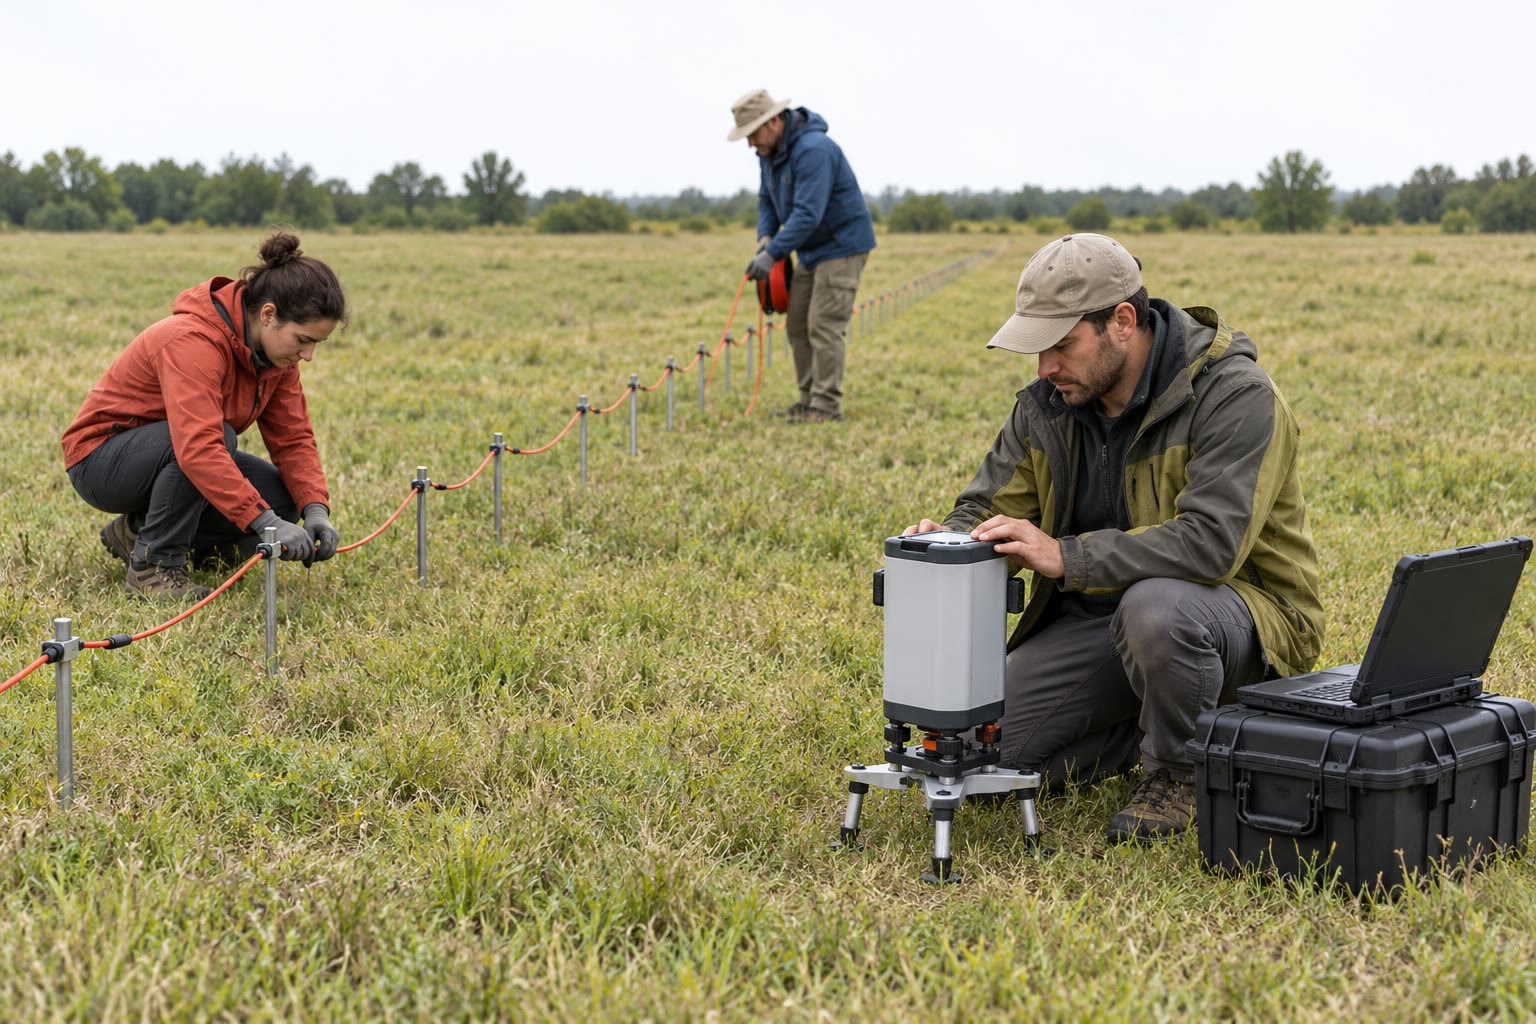
\includegraphics[width=\linewidth]{images/book5/ai/b3-geophysics-crew.jpg}

{\scriptsize Un equipo de geofísica tendiendo un cable de resistividad, con un
gravímetro sobre su base (Ilustración generada por IA.)}
\end{minipage}
\end{inthefield}

\begin{example}[La prospección de Varden]\label{ex:b3:field-lab-methods-3:varden}
El mapa de gravedad muestra un mínimo cerrado de unos \qty{-2.3}{\milli\gal}
centrado sobre el granito, alargado norte--sur: el granito, menos denso,
continúa bajo la cobertera, y es más largo en esa dirección. El mínimo
se extiende unos \qty{1}{km} desde el afloramiento, así que el cuerpo se ensancha con
la profundidad. Su semianchura da una primera profundidad para una esfera equivalente;
los modelos con un flanco vertical y un fondo muestran que un fondo situado entre uno
y unos pocos kilómetros de profundidad explica el máximo igual de bien, con una diferencia de unas
décimas de miligal, así que el fondo queda sin determinar---la no unicidad de
la sección anterior. En el fondo del valle, sobre el granito, el
sondeo parte de la resistividad de la grava seca, desciende donde la
corriente entra en el aluvión saturado de agua y asciende a lo largo de una
recta de pendiente uno: una cobertera conductora sobre un basamento muy resistivo, el
granito, a pocos metros de profundidad. El radar arrastrado por el mismo fondo muestra un
eco plano a unos \qty{20}{ns}: el nivel freático. Y la línea magnética
que cruza el flanco oeste del pliegue, donde la cobertera es gruesa y los
esquistos del basamento yacen a un par de centenares de metros de profundidad, registra un
máximo simétrico de unos \qty{20}{nT} que ningún mapa explica: un dique máfico,
rico en magnetita, enterrado bajo la cobertera; su rumbo a lo largo del
meridiano magnético es la razón de que la anomalía sea simétrica. Los geofísicos
lo describen como un dique de dolerita truncado en la discordancia, que la
cobertera del mapa oculta. El problema de fin de semana reduce los datos de la
prospección.
\end{example}
% ledger: gpg:susceptibility, gpg:resistivity, gpg:gpr-table

\section{Ejercicios}

\begin{exercise}[$\star$]\label{exo:b3:field-lab-methods-3:1}
(a)~¿Qué fracción de $g = \qty{9.81}{m.s^{-2}}$ es \qty{0.01}{\milli\gal}?
(b)~¿Cuánto debe elevarse un gravímetro para que su lectura cambie
en \qty{0.01}{\milli\gal} únicamente por el efecto de aire libre? (c)~¿Y por el efecto de aire libre y el de Bouguer conjuntamente,
con la densidad
\qty{2670}{kg.m^{-3}}?
\end{exercise}

\begin{exercise}[$\star$]\label{exo:b3:field-lab-methods-3:2}
Una esfera de radio \qty{50}{m} y contraste de densidad
\qty{+500}{kg.m^{-3}} tiene su centro a \qty{100}{m} de profundidad. Calcúlense su
exceso de masa, el máximo de su anomalía y la semianchura $x_{1/2}$.
\end{exercise}

\begin{exercise}[$\star$]\label{exo:b3:field-lab-methods-3:3}
Una configuración Wenner de separación $a = \qty{10}{m}$ inyecta \qty{0.1}{A} y
mide \qty{0.239}{V}. (a)~Calcúlense el factor geométrico y la
\omterm{def:b3:field-lab-methods-3:resistivity}{resistividad aparente}. (b)~Demuéstrese que una configuración Schlumberger con $s =
\qty{15}{m}$ y $l = \qty{5}{m}$ tiene el mismo factor geométrico, y
explíquese por qué.
\end{exercise}

\begin{exercise}[$\star$]\label{exo:b3:field-lab-methods-3:4}
El granito tiene $\varepsilon_r = 5$. (a)~Calcúlese la velocidad del radar. (b)~Una
fractura yace a \qty{10}{m} de profundidad: calcúlese el tiempo de ida y vuelta de su eco.
(c)~Con $\sigma = \qty{1}{mS.m^{-1}}$, calcúlense la profundidad de penetración y la
profundidad útil de unas tres profundidades de penetración. (d)~Compárese con una arcilla húmeda de
$\varepsilon_r = 20$ y $\sigma = \qty{10}{mS.m^{-1}}$.
\end{exercise}

\begin{exercise}[$\star\star$]\label{exo:b3:field-lab-methods-3:5}
(a)~Derívese la anomalía de un cilindro horizontal largo de radio $R$ y
contraste de densidad $\Delta\rho$, con su eje a profundidad $z$, a partir de la de una
masa lineal, y demuéstrese que $z = x_{1/2}$. (b)~Un cilindro y una esfera
dan el mismo máximo y la misma semianchura $x_{1/2} = \qty{100}{m}$.
Compárense sus profundidades. ¿Qué interpretación da el cuerpo más profundo?
\end{exercise}

\begin{exercise}[$\star\star$]\label{exo:b3:field-lab-methods-3:6}
La anomalía de Bouguer del modelo de granito de Varden, muestreada cada
\qty{100}{m} en un mapa de \num{1120} puntos que cubre $\qty{3.5}{km}
\times \qty{3.2}{km}$, suma \qty{-438}{\milli\gal}. (a)~Aplíquese la
\cref{prop:b3:field-lab-methods-3:gauss} para estimar el déficit de masa.
(b)~El déficit de masa del modelo es \qty{1.74e11}{kg}. ¿Qué fracción recupera
el mapa, y dónde está el resto?
\end{exercise}

\begin{exercise}[$\star\star$]\label{exo:b3:field-lab-methods-3:7}
(a)~Un dique delgado tiene su techo a \qty{30}{m} de profundidad. Usando la regla de tres
lecturas por semianchura, donde la semianchura es la anchura total de la
anomalía a la mitad de su máximo, ¿qué separación entre estaciones necesita? (b)~Lo
mismo para un techo a \qty{220}{m} de profundidad. (c)~¿Por qué una sola prospección no
puede resolver a la vez un cuerpo somero y uno profundo, a menos que esté diseñada
para el somero?
\end{exercise}

\begin{exercise}[$\star\star$]\label{exo:b3:field-lab-methods-3:8}
Una arenisca saturada de agua de \qty{8}{\ohm\metre} tiene una
resistividad de \qty{80}{\ohm\metre}. (a)~Con $a = 1$ y $m = 2$,
calcúlese su porosidad. (b)~Repítase con $m = 1.8$ y $m = 2.2$. ¿Qué
término de la medida controla la incertidumbre de la porosidad?
\end{exercise}

\begin{exercise}[$\star\star$]\label{exo:b3:field-lab-methods-3:9}
(a)~Calcúlense los tres primeros términos de la serie de dos capas de la
\cref{prop:b3:field-lab-methods-3:layers} para $s = 2h_1$ con $k =
\num{0.5}$ y $k = \num{-0.5}$, y las \omterm{def:b3:field-lab-methods-3:resistivity}{resistividades aparentes} que
dan. (b)~¿Cuáles son los límites de $\rho_a/\rho_1$ para $s \ll h_1$ y
$s \gg h_1$? (c)~¿Qué razones de resistividad $\rho_2/\rho_1$ corresponden a
$k = \pm 0.5$?
\end{exercise}

\begin{exercise}[$\star\star\star$]\label{exo:b3:field-lab-methods-3:10}
(a)~Obténgase el factor geométrico del dispositivo de Wenner a partir
del \cref{thm:b3:field-lab-methods-3:point-source}. (b)~Obténgase el del
dispositivo de Schlumberger y demuéstrese que $\rho_a \to 2\pi s^2(-\mathrm{d}V/
\mathrm{d}r)/I$ cuando $l/s \to 0$. (c)~¿En cuánto sobrestima el factor aproximado
$\pi s^2/(2l)$ al exacto cuando $l = s/10$?
\end{exercise}

\begin{exercise}[$\star\star\star$]\label{exo:b3:field-lab-methods-3:11}
Una estación se encuentra a \qty{50}{m} por encima de la base. Su lectura es buena hasta
\qty{0.01}{\milli\gal}, y su altura, hasta \qty{5}{cm}; la densidad de la
losa tiene una incertidumbre de \qty{100}{kg.m^{-3}}, y la \omterm{def:b3:field-lab-methods-3:terrain}{corrección topográfica}, de
\qty{0.2}{\milli\gal}. (a)~Elabórese el presupuesto de error de su
anomalía de Bouguer. (b)~¿Qué término domina, y cuál mejoraría para
detectar una anomalía de \qty{0.1}{\milli\gal}? (c)~¿Cuál es el total sin
el término topográfico?
\end{exercise}

\begin{exercise}[$\star\star\star$]\label{exo:b3:field-lab-methods-3:12}
Cinco lecturas gravimétricas a lo largo de un cuerpo enterrado, en $x = -600$, $-300$, $0$,
$300$ y \qty{600}{m}, son \num{-0.69}, \num{-2.17}, \num{-4.16},
\num{-2.10} y \qty{-0.73}{\milli\gal}, cada una con $\sigma =
\qty{0.03}{\milli\gal}$. (a)~Para modelos de esfera centrados bajo $x = 0$ a
profundidades de \num{300}, \num{400} y \qty{500}{m}, elíjase la masa que
ajuste la lectura central y calcúlese el \omterm{def:b3:field-lab-methods-3:inversion-practice}{desajuste} $\chi^2$ de cada uno. (b)~¿Qué
modelo ajusta los datos dentro de sus errores? (c)~¿Podría ajustar igual de bien un cuerpo de otra
forma? ¿Qué lo decidiría?
\end{exercise}

\section{Problema: los cuerpos ocultos de las colinas de Varden}

\begin{problem}[{Problema de fin de semana --- reducción del levantamiento de Varden}]
\label{pb:b3:field-lab-methods-3:1}
Utilícense $G = \qty{6.674e-11}{m^3.kg^{-1}.s^{-2}}$, el gradiente de aire libre
\qty{0.3086}{\milli\gal.m^{-1}} y el factor de Bouguer
\qty{0.1119}{\milli\gal.m^{-1}} (densidad \qty{2670}{kg.m^{-3}}).

\medskip\noindent\textbf{Parte I --- Un circuito gravimétrico.} Un circuito sobre el
perfil gravimétrico da (lecturas en miligales tras la calibración, alturas
en metros, tiempos en horas después de las 09:00):
\begin{center}
\small
\begin{tabular}{lccccc}
\hline
estación & base & \qty{3.0}{km} & \qty{3.5}{km} & \qty{4.0}{km} & base \\
\hline
tiempo & 0 & 0.5 & 0.9 & 1.3 & 2.0 \\
altura & 176.1 & 149.0 & 145.5 & 158.0 & 176.1 \\
lectura & 2846.512 & 2851.075 & 2850.497 & 2849.392 & 2846.708 \\
\hline
\end{tabular}
\end{center}
\begin{enumerate}
\item Calcúlese la tasa de deriva del circuito.
\item Corríjanse las tres lecturas de las estaciones por la deriva y exprésense
  respecto a la base.
\item Apliquense las correcciones de aire libre y de Bouguer por las
  diferencias de altura, y dése la anomalía de Bouguer de cada estación respecto a
  la base.
\item La deriva del instrumento por sí sola fue de \qty{0.040}{\milli\gal.h^{-1}}.
  ¿Qué causó el resto del cambio en la base, y por qué podría eliminarse con la
  deriva?
\item El modelo del que proceden las lecturas da las tres anomalías
  respecto a la base como \num{-0.825}, \num{-2.131} y
  \qty{-0.825}{\milli\gal}. Calcúlense los errores de la reducción. Las
  alturas de la tabla están redondeadas a \qty{0.1}{m}: ¿qué error puede introducir
  este redondeo, y si explica los errores?
\item ¿Qué precisión en la altura mantiene la anomalía reducida dentro de
  \qty{0.01}{\milli\gal}? ¿Por qué los manuales de levantamiento piden
  \qty{3.3}{cm}, una cifra más exigente?
\end{enumerate}

\medskip\noindent\textbf{Parte II --- La anomalía del granito.} A lo largo
del perfil la anomalía tiene su mínimo, \qty{-2.293}{\milli\gal}, en
$x = \qty{3.50}{km}$, y cruza la mitad de ese valor en $x = 3.048$ y
\qty{3.952}{km}. El modelo de granito tiene un contraste de densidad de
\qty{-130}{kg.m^{-3}}, y el terreno en el centro está a \qty{145.5}{m}
sobre el nivel del mar.
\begin{enumerate}[resume]
\item Calcúlense la semianchura $x_{1/2}$ y la profundidad del centro de
  la esfera equivalente.
\item Calcúlese el déficit de masa de esa esfera, y su radio para el
  contraste de densidad del granito. ¿Qué tiene de extraño el resultado?
\item El centro de masa del modelo está a \qty{864}{m} bajo el terreno y su
  déficit de masa es \qty{1.74e11}{kg}. ¿Por qué la regla de la semianchura da un
  cuerpo más somero y más ligero?
\item Un cilindro vertical de la misma área que el granito en la
  discordancia tiene un radio de \qty{461}{m}. Calcúlese su anomalía sobre el eje
  para un techo en el terreno y un fondo a \qty{1645}{m} de profundidad, y para una
  profundidad ilimitada.
\item Encuéntrese, por tanteo o resolviendo, la profundidad del fondo para la que
  este cilindro da la anomalía observada de \qty{-2.29}{\milli\gal}.
\item Calcúlese la anomalía del cilindro con su techo \qty{6}{m} por debajo
  (fondo a \qty{1645}{m}). ¿Puede la gravedad distinguir si el granito llega a la
  superficie bajo el aluvial?
\end{enumerate}

\medskip\noindent\textbf{Parte III --- El fondo del valle.} El sondeo de Schlumberger
en el fondo sobre el granito da (semiseparación $s$ en
metros, $\rho_a$ en \unit{\ohm\metre}):
\begin{center}
\small
\begin{tabular}{lcccccccc}
\hline
$s$ & 1 & 2 & 4 & 6 & 10 & 20 & 30 & 40 \\
$\rho_a$ & 577 & 526 & 387 & 350 & 449 & 821 & 1309 & 1684 \\
\hline
\end{tabular}
\end{center}
En un perfil de radar a lo largo del mismo fondo, una tubería da una hipérbola con
su vértice a \qty{10.7}{ns} y un tiempo de \qty{17.1}{ns} a \qty{1}{m}
de distancia; un eco plano llega a \qty{20.0}{ns}.
\begin{enumerate}[resume]
\item Con $s = \qty{20}{m}$, MN medía \qty{2}{m} de longitud y la corriente
  \qty{50}{mA}. Calcúlese el factor geométrico y la tensión medida.
\item Calcúlese la velocidad del radar, la permitividad relativa del
  aluvial y la profundidad de la tubería.
\item El eco plano es el nivel freático. ¿A qué profundidad está?
\item Estímese la conductancia $S$ del aluvial a partir de las lecturas a
  20, 30 y \qty{40}{m}.
\item El aluvial seco tiene \qty{600}{\ohm\metre}, y el aluvial
  saturado \qty{222}{\ohm\metre}. Calcúlese el espesor del aluvial saturado
  y la profundidad del techo del granito. ¿Es la estimación alta
  o baja, y por qué?
\item El agua subterránea tiene \qty{20}{\ohm\metre}. Calcúlese la porosidad del
  aluvial mediante la \omterm{prop:b3:field-lab-methods-3:archie}{ley de Archie} con $m = 2$, y el intervalo de $m$
  entre \num{1.3} y \num{2.8}.
\end{enumerate}

\medskip\noindent\textbf{Parte IV --- La línea magnética.} La línea avanza
hacia el este desde $x = \qty{1.70}{km}$, con una estación cada \qty{50}{m} y
cada dos minutos; la estación base registró en los mismos minutos. Las
lecturas, menos \qty{48000}{nT}, son:
\begin{center}
\small
\setlength{\tabcolsep}{3.5pt}
\begin{tabular}{lccccccccccc}
\hline
$x$ (km) & 1.70 & 1.75 & 1.80 & 1.85 & 1.90 & 1.95 & 2.00 & 2.05 & 2.10 & 2.15 & 2.20 \\
línea & 3.4 & 4.8 & 6.3 & 8.1 & 10.3 & 12.8 & 15.8 & 19.2 & 22.9 & 26.2 & 28.0 \\
base & 0.0 & 0.7 & 1.5 & 2.2 & 2.9 & 3.6 & 4.3 & 5.0 & 5.7 & 6.4 & 7.0 \\
\hline
$x$ (km) & 2.25 & 2.30 & 2.35 & 2.40 & 2.45 & 2.50 & 2.55 & 2.60 & 2.65 & 2.70 & \\
línea & 27.7 & 25.8 & 23.3 & 20.9 & 19.0 & 17.6 & 16.6 & 15.9 & 15.5 & 15.2 & \\
base & 7.6 & 8.2 & 8.8 & 9.4 & 9.9 & 10.4 & 10.9 & 11.3 & 11.7 & 12.1 & \\
\hline
\end{tabular}
\end{center}
El campo principal es de \qty{48000}{nT}, con una inclinación de \ang{65}.
\begin{enumerate}[resume]
  \item Aplíquese la \omterm{def:b3:field-lab-methods-3:magnetic}{corrección diurna} y dese la anomalía corregida en
  cada estación.
  \item Demuéstrese que, sin la corrección, la anomalía nunca desciende a la
  mitad de su máximo en el lado este.
  \item Localícese el pico y los dos puntos donde la anomalía corregida vale
  la mitad del pico, por interpolación lineal, y calcúlese la semianchura.
  \item La anomalía es simétrica. ¿Qué indica esto sobre el rumbo del
  cuerpo, y qué tipo de cuerpo supone la regla de la semianchura?
  \item Calcúlese el producto $\kappa t$ de la susceptibilidad y el espesor.
  Si el dique es una dolerita de susceptibilidad \num{0.03}, ¿qué espesor
  tiene?
  \item ¿Estaban las estaciones suficientemente próximas?
  \item Dese la profundidad del techo del dique oculto bajo el suelo, con
  aproximación de diez metros, y compárese con la profundidad de la
  discordancia en el modelo geológico de la región, \qty{222}{m} en este
  punto.
\end{enumerate}
\end{problem}
% ledger: gpg:grav-survey, gpg:mag-field, keys:archie
